% =============================================================================
%  Section 3.3 - Thiết kế tầng xử lý GraphRAG
%  Subsections:
%    3.3.1  Thiết kế phân hệ G-Retrieval
%      - Tiền xử lý và trích xuất thực thể
%      - Truy vấn đa mức độ
%      - Tổ chức ngữ cảnh
%    3.3.2  Thiết kế phân hệ G-Generation
%      - Xây dựng cấu trúc Prompt
%      - Các chiến lược tạo sinh
% =============================================================================

\section{Thiết kế tầng xử lý GraphRAG}

\subsection{Thiết kế phân hệ G-Retrieval}
\label{sec:g_retrieval}

Phân hệ G-Retrieval chịu trách nhiệm xác định và trích xuất phần thông tin phù hợp từ đồ thị tri thức để cung cấp ngữ cảnh cho quá trình tạo sinh câu trả lời. Trong hệ thống GraphRAG được đề xuất, chất lượng câu trả lời phụ thuộc trực tiếp vào chất lượng ngữ cảnh được truy xuất, vì vậy nên thiết kế của phân hệ này đóng vai trò quyết định đối với hiệu năng tổng thể của toàn hệ thống.

Phân hệ G-Retrieval được tổ chức thành ba giai đoạn xử lý tuần tự (Hình~\ref{fig:g_retrieval_overview}): (1) tiền xử lý và trích xuất thực thể, (2) truy vấn đa mức độ, và (3) tổ chức ngữ cảnh. Đầu vào tổng thể của phân hệ là câu hỏi ngôn ngữ tự nhiên $q$ từ người dùng; đầu ra là tập ngữ cảnh đã được định dạng $C = \{(f_i, text_i)\}$, trong đó $f_i$ là định dạng biểu diễn và $text_i$ là nội dung văn bản tương ứng. Cùng với $C$, giai đoạn này còn đưa ra tập dữ kiện chính $K$ (key facts) - các mệnh đề ngắn tóm lược những thông tin quan trọng nhất từ kết quả truy xuất - được dùng bổ trợ cho phân hệ G-Generation.

\begin{figure}[!ht]
  \centering
  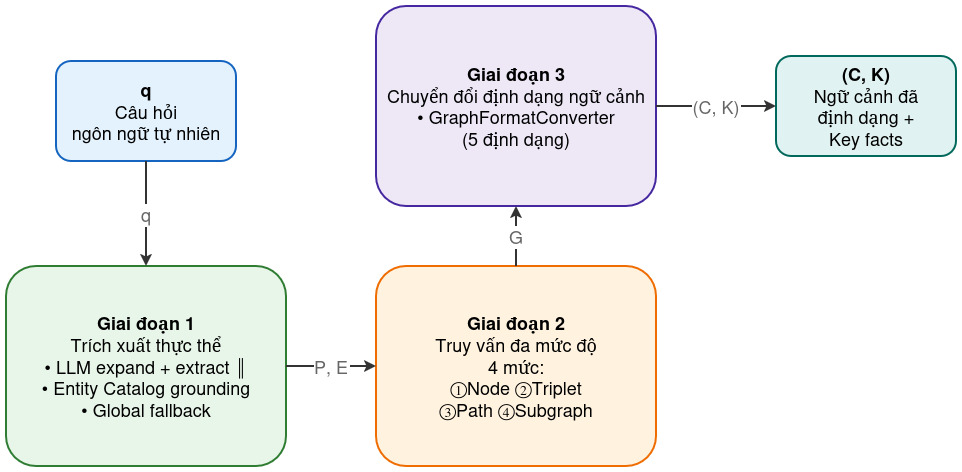
\includegraphics[width=\textwidth]{figures/c3/g_retrieval_overview.jpg}
  \caption{Sơ đồ tổng quan phân hệ G-Retrieval.}
  \label{fig:g_retrieval_overview}
\end{figure}


\subsubsection{Tiền xử lý và trích xuất thực thể}

Giai đoạn đầu tiên của phân hệ G-Retrieval có nhiệm vụ mở rộng/phân rã truy vấn gốc, từ đó xác định các thực thể liên quan trong đồ thị tri thức. Để giảm độ trễ, hai tiến trình gọi LLM được thực hiện \textit{song song} (Hình~\ref{fig:entity_extraction}), đưa độ trễ tổng về mức $\max(t_A, t_B)$ thay vì $t_A + t_B$.

\textbf{Đầu vào.} Câu hỏi ngôn ngữ tự nhiên $q$ từ người dùng. Ví dụ:

\begin{tcolorbox}[colback=gray!5, colframe=black!50, arc=4pt, boxrule=0.5pt]
{\small
\begin{verbatim}
q = "Ai đóng vai Thị Màu trong vở Quan Âm Thị Kính?"
\end{verbatim}
}
\end{tcolorbox}

\textbf{Tiến trình A - Mở rộng truy vấn và trích xuất thực thể.} Hệ thống tiến hành gọi tới LLM với câu hỏi gốc $q$ đi cùng với \textbf{danh mục thực thể} (Mục~\ref{sec:entity_catalog}) với mục đích yêu cầu LLM thực hiện hai nhiệm vụ. Thứ nhất, LLM cần mở rộng $q$ thành truy vấn $q'$ với khả năng khai thác ngữ cảnh nghệ thuật Chèo sâu rộng hơn, từ đó trích xuất các thực thể từ câu hỏi $q'$ vào tập $E_A$ - tập thực thế được phân loại theo bốn nhóm \textit{characters}, \textit{actors}, \textit{plays}, \textit{scenes}. Trong câu prompt yêu cầu tới LLM có đặt thêm yếu tố ràng buộc ``chỉ chọn thực thể có trong Danh mục''  nhằm đảm bảo các thực thể mà LLM chọn ra thực sự tồn tại trong đồ thị tri thức, tránh được hiện tượng ảo giác thông tin không mong muốn. Cùng lượt gọi này, LLM còn phân loại câu hỏi vào một trong ba mức $t \in \{\textit{Local}, \textit{Community}, \textit{Global}\}$ làm tín hiệu định tuyến cho các giai đoạn sau.

\textbf{Tiến trình B - Phân rã truy vấn và trích xuất bổ sung.} Song song với tiến trình A, hệ thống cũng gọi LLM thêm một lượt nữa nhằm phân rã $q$ thành các câu hỏi con $\{q_1, \ldots, q_n\}$ - mỗi câu hỏi con tập trung vào một khía cạnh đơn lẻ, chẳng hạn ``Ai đóng vai Thị Màu trong vở Quan Âm Thị Kính?'' tách thành ``Thị Màu là nhân vật như thế nào?'', ``Vở Quan Âm Thị Kính có những diễn viên nào?'' và ``Ai đóng vai Thị Màu?'' - rồi trích xuất thực thể trên từng câu hỏi con thành tập $E_B$ (có sự ràng buộc thực thể tương tự tiến trình A''. 

Sau khi cả hai tác vụ hoàn thành, hệ thống chọn ra tập thực thể phù hợp nhất bằng phép hợp $E = E_A \cup E_B$ và có sự loại bỏ trùng lặp: A bắt thực thể có tên hiển thị trực tiếp trong câu hỏi gốc, B bắt thực thể bị che bởi cách diễn đạt phức tạp - hai góc nhìn bổ sung nhau giúp tăng độ phủ mà không sinh ra các thực thể ảo, vì các thực thể này vốn đã được trích xuất dưới sự ràng buộc của danh mục thực thể.

Hệ thống đồng thời hỗ trợ một \textit{chế độ đơn giản} dành cho tình huống cần giảm chi phí khi gọi LLM. Khi câu hỏi ngắn gọn, rõ ràng, hệ thống sẽ chọn chế độ đơn giản, bỏ qua 2 tác vụ song song mà trực tiếp trích xuất thực thể từ câu hỏi gốc $q$. 

\textbf{Đầu ra.} Giai đoạn tiền xử lý tạo ra ba đối tượng:
\begin{itemize}
  \item Đối tượng \textit{ProcessedQuery} $Q = (q,\ q',\ \{q_1, \ldots, q_n\})$, gồm truy vấn gốc, truy vấn mở rộng và tập câu hỏi con.
  \item Tập thực thể $E = E_A \cup E_B$ phân loại theo bốn nhóm \textit{characters}, \textit{actors}, \textit{plays}, \textit{scenes}, hợp nhất từ hai tác vụ và đã được chuẩn hoá về tên định danh trong Danh mục thực thể. Đây là đầu vào trực tiếp cho giai đoạn truy xuất đồ thị tiếp theo.
  \item Nhãn loại truy vấn $t \in \{\textit{Local}, \textit{Community}, \textit{Global}\}$, đóng vai trò tín hiệu định tuyến để chọn tập mức truy xuất (Mục~\ref{sec:multi_granularity}) và lựa chọn chiến lược tạo sinh (Mục~\ref{sec:g_generation}).
\end{itemize}

\begin{tcolorbox}[colback=gray!5, colframe=black!50, arc=4pt, boxrule=0.5pt]
{\small
\begin{verbatim}
Q = {
  original:   "Ai đóng vai Thị Màu
               trong vở Quan Âm Thị Kính?",
  expanded:   "Diễn viên nào đảm nhận vai diễn
               nhân vật Thị Màu trong vở chèo
               Quan Âm Thị Kính?",
  decomposed: [
    "Thị Màu là nhân vật trong vở nào?",
    "Ai đóng vai Thị Màu?"
  ]
}

E = {
  characters: ["Thị Màu"],
  actors: [],
  plays: ["Quan Âm Thị Kính"],
  scenes: []
}

t = "Local"
\end{verbatim}
}
\end{tcolorbox}

\begin{figure}[!ht]
  \centering
  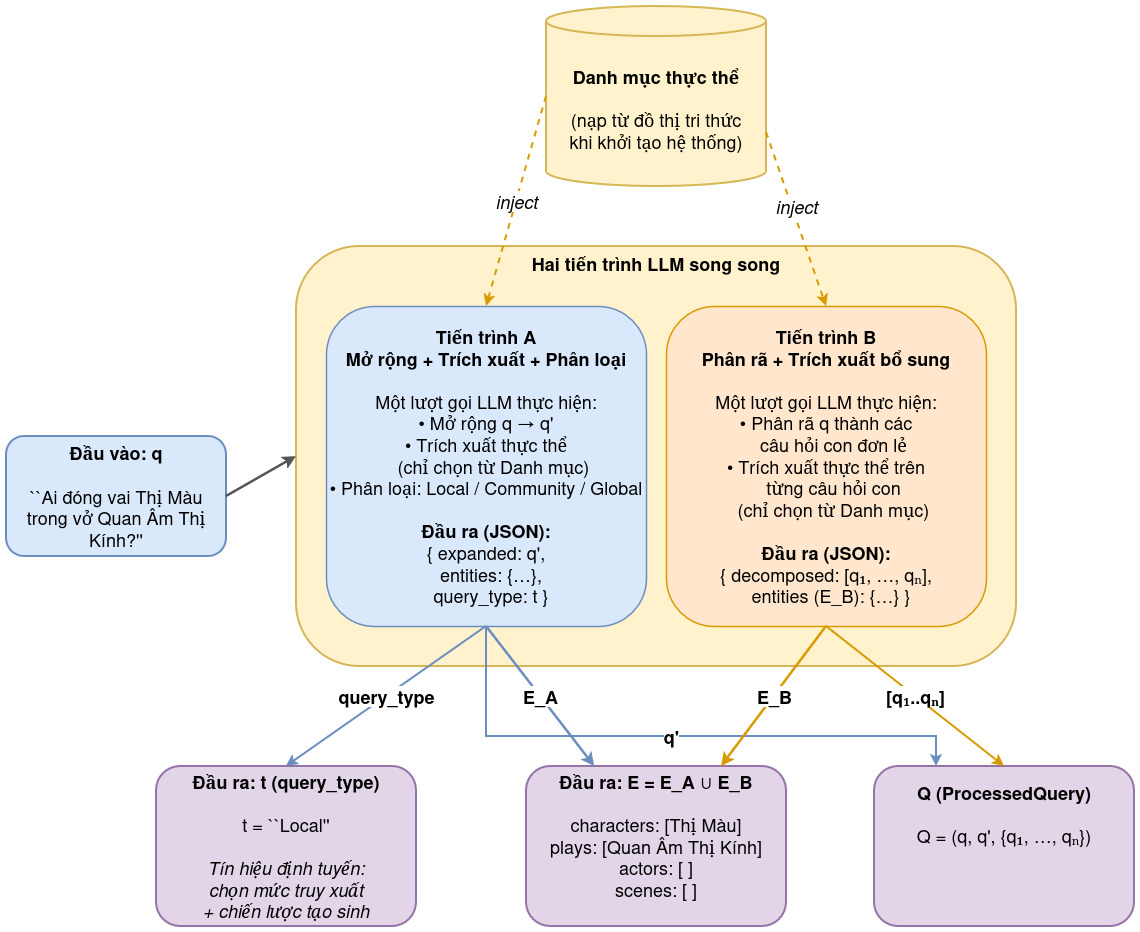
\includegraphics[width=\textwidth]{figures/c3/entity_extraction.jpg}
  \caption{Quy trình trích xuất thực thể song song.}
  \label{fig:entity_extraction}
\end{figure}


\subsubsection{Truy vấn đa mức độ}
\label{sec:multi_granularity}

Giai đoạn thứ hai trong phân hệ G-Retrieval thực hiện truy xuất tri thức từ đồ thị tri thức dựa trên tập thực thể đã trích xuất $E$. Thông thường, một câu hỏi về nhân vật đơn lẻ sẽ yêu cầu mức độ thông tin ít hơn so với những câu hỏi có sự tổng hợp xuyên suốt nhiều vở diễn, nên nếu hệ thống chỉ dùng một cách truy xuất duy nhất, câu trả lời dễ rơi vào một trong hai tình huống: thiếu thông tin khi mức độ truy xuất quá nông, hoặc nhiễu tràn lan khi phạm vi truy xuất quá rộng. Phân hệ G-Retrieval vì vậy tổ chức \textbf{bốn mức độ truy xuất} (Hình~\ref{fig:multi_granularity}), mỗi mức khai thác một khía cạnh khác nhau trong cấu trúc đồ thị.

\begin{figure}[!ht]
  \centering
  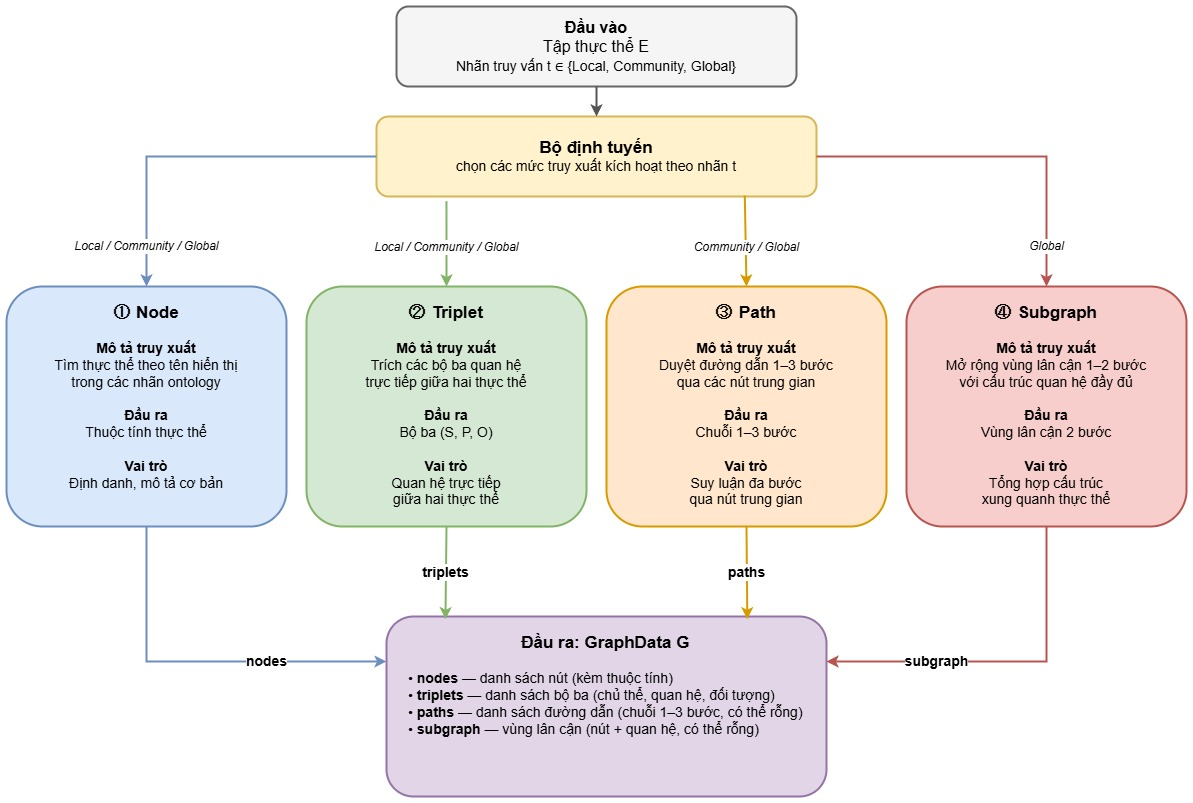
\includegraphics[width=0.9\textwidth]{figures/c3/multi_granularity.jpg}
  \caption{Bốn mức truy xuất trong G-Retrieval.}
  \label{fig:multi_granularity}
\end{figure}

\textbf{Đầu vào.} Tập thực thể $E$ và nhãn loại truy vấn $t$ từ giai đoạn tiền xử lý.

\begin{table}[ht]
  \centering
  \caption{Bốn mức độ truy xuất trong phân hệ G-Retrieval.}
  \label{tab:retrieval_levels}
  \resizebox{\textwidth}{!}{%
  \begin{tabular}{c p{5.6cm} l p{4.2cm}}
    \hline
    \textbf{Mức} & \textbf{Mô tả truy xuất} & \textbf{Đầu ra} & \textbf{Vai trò} \\
    \hline
    \textcircled{1} Node & Tìm thực thể theo tên hiển thị trong các nhãn ontology & Thuộc tính thực thể & Định danh, mô tả cơ bản \\
    \textcircled{2} Triplet & Trích các bộ ba quan hệ trực tiếp giữa hai thực thể & Bộ ba (S, P, O) & Quan hệ trực tiếp giữa hai thực thể \\
    \textcircled{3} Path & Duyệt đường dẫn 1-3 bước qua các nút trung gian & Chuỗi 1-3 bước & Suy luận đa bước qua trung gian \\
    \textcircled{4} Subgraph & Mở rộng vùng lân cận 1-2 bước với cấu trúc quan hệ đầy đủ & Vùng lân cận 2 bước & Tổng hợp cấu trúc xung quanh thực thể \\
    \hline
  \end{tabular}%
  }
\end{table}

\textbf{Mô tả các mức truy xuất.} Bốn mức truy xuất (Bảng~\ref{tab:retrieval_levels}) được mô tả lần lượt dưới đây, the thứ tự tăng dần về độ phức tạp.

\textit{Mức Node.} Truy vấn được thực hiện dựa trên bốn nhãn gốc của ontology - Character, Actor, Play, Scene - bằng các sử dụng các trường tên hiển thị; các nhãn con của Character (Đào, Hề, Kép, Mụ, Lão và các subType ở Mục~\ref{sec:schema_extension}) được bao phủ gián tiếp nhờ kế thừa từ nhãn gốc. Để giảm chi phí, tên các thực thể trong tập $E$ được gộp lại và thực hiện truy vấn cùng một lượt tới cơ sở dữ liệu; khi không khớp chính xác, hệ thống chuyển sang tìm kiếm mờ trên trường tên nhằm xử lý các biến thể chính tả thường gặp. Mỗi nút trả về kèm theo đầy đủ thuộc tính riêng - id, tên hiển thị, vai trò, mô tả ngắn - phần tri thức của thực thể khi đứng một mình, chưa gắn với bất kỳ liên kết nào tới các thực thể khác.

\textit{Mức Triplet.} Tổng cộng tám mẫu truy vấn được phân thành ba nhóm theo loại tri thức mà chúng mang lại. Nhóm thứ nhất gồm các quan hệ vai diễn cốt lõi: Character $\leftrightarrow$ Actor thông qua RoleAssignment, Play $\rightarrow$ Character qua \texttt{HAS\_CHARACTER}, và Play $\rightarrow$ Scene qua \texttt{HAS\_SCENE} - bộ ba này phủ các câu hỏi cơ bản dạng ``ai đóng vai gì trong vở nào''. Nhóm thứ hai là các quan hệ phái sinh xuyên thực thể, trong đó một số chuỗi nhiều bước được rút gọn sẵn thành cạnh trực tiếp nhằm tránh để LLM phải tự nối ghép, gồm Actor $\rightarrow$ Play qua \texttt{PERFORMS\_IN} (rút gọn từ chuỗi năm bước RoleAssignment-Version-Scene-Play), RoleAssignment $\rightarrow$ Version qua \texttt{IN\_VERSION} kèm tên phiên bản hiển thị, và RoleAssignment $\rightarrow$ Appearance kèm cảm xúc cùng lời thoại của lần xuất hiện. Nhóm thứ ba khai thác các lớp biểu hiện diễn xuất bổ sung trong schema mở rộng (Mục~\ref{sec:schema_extension}), gồm Actor $\rightarrow$ Mood qua \texttt{EXPRESS}, Costume $\rightarrow$ Actor qua \texttt{IS\_WEAR\_BY}, và Character $\rightarrow$ Costume qua \texttt{WEARS\_COSTUME} - cả ba phục vụ các câu hỏi về cảm xúc và trang phục theo vai diễn. Khi cả tám mẫu đều không trả về kết quả, hệ thống lấy mẫu một số bộ ba quan hệ diễn viên-nhân vật tiêu biểu từ đồ thị làm dự phòng.

\textit{Mức Path.} Đường dẫn xuất phát từ các thực thể trong tập $E$ thuộc nhóm Character, Actor hoặc Play, đi qua các nút trung gian rồi kết thúc tại một trong bốn nhóm thực thể chính. Tên hiển thị của tất cả các nút dọc theo đường dẫn được nối thành chuỗi tuyến tính dạng ``Thị Màu $\rightarrow$ RoleAssignment $\rightarrow$ Version: \ldots $\rightarrow$ Quan Âm Thị Kính'' - từ đó mô tả cả những nút trung gian như RoleAssignment hay Version vốn không xuất hiện trong tập $E$ ban đầu. Mỗi chuỗi như vậy có tác dụng tạo nên một mạch suy luận tường minh, giúp LLM theo dõi được cách hai thực thể được nối với nhau qua trung gian thay vì phải tự ghép nối từ các bộ ba rời rạc. Các nút trung gian ấy cũng trở thành cơ sở 
để LLM ghép nối các đường dẫn, tạo nên một mạng lưới thông tin nhỏ cung cấp tri thức về đối tượng cần truy xuất.

\textit{Mức Subgraph.} Vùng đồ thị con xung quanh mỗi thực thể trung tâm trong tập $E$ được thu thập đồng thời cả nút lẫn quan hệ - vừa lưu lại thuộc tính chi tiết của từng nút trong vùng lân cận, vừa bảo toàn kiểu của các cạnh nối giữa chúng. Cấu trúc đầu ra vì thế là một bản sao thu nhỏ của lát cắt đồ thị xung quanh thực thể, phù hợp với những câu trả lời đòi hỏi tổng hợp hoặc so sánh trên nhiều thực thể có quan hệ đan xen, khi LLM cần đồng thời cả nút lẫn liên kết để đưa ra nhận định toàn cục.

\textbf{Định tuyến theo loại truy vấn.} Tập mức được kích hoạt phụ thuộc trực tiếp vào nhãn $t$ do Tiến trình A trả về theo quy tắc ánh xạ (Bảng~\ref{tab:level_mapping}). Ánh xạ này được thiết kế theo nguyên tắc tăng tiến: câu hỏi càng đòi hỏi suy luận sâu hoặc tổng hợp rộng thì càng cần thêm các mức đi xa hơn về cấu trúc đồ thị, còn các mức không cần thiết được lược bỏ. Nhờ đó, nhãn $t$ đóng vai trò chuyển hệ thống từ chế độ ``chạy tất cả'' sang chế độ ``chạy đúng những gì cần'' - vừa giúp kiểm soát kích thước ngữ cảnh và chi phí truy vấn, vừa tránh đưa các mức không phù hợp vào prompt làm pha loãng thông tin cốt lõi.

\begin{table}[ht]
  \centering
  \caption{Ánh xạ mức truy xuất theo loại truy vấn.}
  \label{tab:level_mapping}
  \resizebox{\textwidth}{!}{%
  \begin{tabular}{l l l}
    \hline
    \textbf{Loại truy vấn} & \textbf{Mức kích hoạt} & \textbf{Ví dụ} \\
    \hline
    Local      & Node, Triplet                 & ``Ai đóng vai Thị Màu?'' \\
    Community  & Node, Triplet, Path           & ``Diễn viên nào đóng cả Quan Âm Thị Kính lẫn Kim Nham?'' \\
    Global     & Node, Triplet, Path, Subgraph & ``So sánh số phận Súy Vân và Thị Kính'' \\
    \hline
  \end{tabular}%
  }
\end{table}

\textbf{Đầu ra.} Đối tượng dữ liệu đồ thị $G$ (Hình~\ref{fig:multi_granularity}) hợp nhất kết quả từ các mức được kích hoạt, gồm bốn trường tương ứng với bốn mức truy xuất. Tiếp tục với câu hỏi ví dụ ban đầu - $q$ = ``Ai đóng vai Thị Màu trong vở Quan Âm Thị Kính?'', $E = \{\text{Thị Màu}, \text{Quan Âm Thị Kính}\}$, $t = \textit{Local}$ - đầu ra cụ thể có dạng:

\begin{tcolorbox}[colback=gray!5, colframe=black!50, arc=4pt, boxrule=0.5pt]
{\small
\begin{verbatim}
G = {
  nodes: [
    {id: "Thị Màu",
     label: "Character",
     roleType: "Đào",
     description: "Nhân vật nữ chính ..."},
    {id: "Quan Âm Thị Kính",
     label: "Play",
     description: "Vở chèo kinh điển ..."}
  ],
  triplets: [
    ("Quan Âm Thị Kính", "HAS_CHARACTER", "Thị Màu"),
    ("Thị Màu",          "PERFORMED_BY",  "Vân Quyền"),
    ("Quan Âm Thị Kính", "HAS_SCENE",     "Thị Màu lên chùa")
  ],
  paths:    [],   // không kích hoạt vì t = Local
  subgraph: []    // không kích hoạt vì t = Local
}
\end{verbatim}
}
\end{tcolorbox}

Cấu trúc đồng nhất bốn trường - dù một số trường có thể rỗng tuỳ $t$ - giúp giai đoạn tổ chức ngữ cảnh tiếp theo biết chính xác phần dữ liệu nào sẵn có để chọn định dạng biểu diễn phù hợp.

\subsubsection{Tổ chức ngữ cảnh}

Giai đoạn cuối cùng của phân hệ G-Retrieval đảm nhận hai nhiệm vụ song song: chuyển đổi dữ liệu đồ thị thô $G$ thành các biểu diễn văn bản phù hợp với mô hình ngôn ngữ, và trích xuất tập dữ kiện chính làm cơ sở cho quá trình tạo sinh.

\textbf{Đầu vào.} Dữ liệu đồ thị $G$ từ giai đoạn truy xuất.

Khác với kiểu văn bản tuần tự thông thường, $G$ chứa thông tin ở nhiều cấp độ cấu trúc - từ thực thể đơn lẻ tới các chuỗi liên kết và các cụm đồ thị con, nên cần có một cơ chế chuyển đổi thông tin phù hợp để LLM có thể tận dụng tối đa lượng tri thức này. Một cách biểu diễn duy nhất không thể truyền tải đầy đủ tri thức trong $G$ cho LLM, do đó bộ chuyển đổi định dạng sinh ra bốn biểu diễn văn bản riêng biệt (Hình~\ref{fig:context_organization}), mỗi biểu diễn khai thác một khía cạnh khác nhau của $G$.

\textbf{Các định dạng biểu diễn.} Bốn định dạng không tương ứng một-một với bốn mức truy xuất, mà chia thành hai nhóm theo phạm vi dữ liệu mà chúng bao phủ. Hai định dạng \textit{đa năng} - \texttt{natural\_language} và \texttt{code\_like} - đọc kết quả từ nhiều mức cùng lúc, phù hợp khi $G$ có dữ liệu từ nhiều mức được kích hoạt. Hai định dạng \textit{chuyên biệt} - \texttt{adjacency\_table} cho mức Triplet và \texttt{node\_sequence} cho mức Path - bám sát cấu trúc của đúng một mức.

\textit{Định dạng natural\_language.} Mỗi bộ ba quan hệ trong $G$ được chuyển thành một câu tiếng Việt hoàn chỉnh, trong đó tên các quan hệ kỹ thuật được đổi thành cụm từ tiếng Việt tương ứng - chẳng hạn \texttt{HAS\_CHARACTER} thành ``có nhân vật'', \texttt{PERFORMED\_BY} thành ``được đóng bởi''. Định dạng này gộp dữ liệu từ ba mức cùng một lúc - thuộc tính nút (Node), bộ ba (Triplet) và các cạnh trong vùng lân cận (Subgraph) - phù hợp với những câu hỏi mà câu trả lời có thể rút ra từ vài bộ ba độc lập.

\vspace{0.5em}
\begin{tcolorbox}[colback=gray!5, colframe=black!50, arc=4pt, boxrule=0.5pt, left=4pt, right=4pt, top=4pt, bottom=4pt, boxsep=0pt]
\small \texttt{"Nhân vật Thị Màu thuộc vở diễn Quan Âm Thị Kính. Nhân vật Thị Màu được thể hiện bởi diễn viên Vân Quyền."}
\end{tcolorbox}

\textit{Định dạng adjacency\_table.} Tập bộ ba quan hệ được trình bày dưới dạng bảng Markdown ba cột - Nút khởi đầu, Loại quan hệ, Nút đích - mỗi dòng tương ứng một bộ ba. Định dạng này phù hợp với các câu hỏi cần đối chiếu nhiều quan hệ cùng lúc, khi cấu trúc bảng giúp LLM tìm từng quan hệ trong một tập hợp dữ liệu với nhiều quan hệ đan xen nhau.

\vspace{0.5em}
\begin{tcolorbox}[colback=gray!5, colframe=black!50, arc=4pt, boxrule=0.5pt, left=4pt, right=4pt, top=4pt, bottom=4pt, boxsep=0pt]
\small
\begin{verbatim}
| Nút Khởi Đầu     | Loại Quan Hệ   | Nút Đích          |
|------------------|----------------|-------------------|
| Quan Âm Thị Kính | HAS_CHARACTER  | Thị Màu           |
| Thị Màu          | PERFORMED_BY   | Vân Quyền         |
\end{verbatim}
\end{tcolorbox}

\textit{Định dạng code\_like.} Toàn bộ đối tượng $G$ - gồm cả bốn mức độ truy xuất \texttt{nodes}, \texttt{triplets}, \texttt{paths} và \texttt{subgraph} - được đóng gói thành cấu trúc JSON, giữ nguyên thuộc tính và nhãn ontology của từng nút cũng như kiểu của từng cạnh quan hệ. Định dạng này giữ nguyên dữ liệu của cả bốn mức, phù hợp với các câu hỏi cần phân tích thuộc tính chi tiết của nhiều thực thể có liên kết phức tạp - khi việc giữ nguyên schema gốc giúp LLM tra cứu chính xác từng nút và cạnh. Thay vì cố gắng tái tổ chức lại hệ thống tri thức dày đặc của các \texttt{subgraph}, LLM được cung cấp dưới dạng JSON như một bản mô tả tóm tắt về cơ sở dữ liệu đang có, phù hợp với các xử lý thông tin và suy luận của chúng.

\vspace{0.5em}
\begin{tcolorbox}[colback=gray!5, colframe=black!50, arc=4pt, boxrule=0.5pt, left=4pt, right=4pt, top=4pt, bottom=4pt, boxsep=0pt]
\small
\begin{verbatim}
{
  "nodes": [
    {"id": "Quan Âm Thị Kính", "label": "Play"},
    {"id": "Thị Màu",          "label": "Character"},
    {"id": "Vân Quyền",        "label": "Actor"}
  ],
  "relationships": [
    {"start": "Quan Âm Thị Kính", "type": "HAS_CHARACTER",
     "end": "Thị Màu"},
    {"start": "Thị Màu",          "type": "PERFORMED_BY",
     "end": "Vân Quyền"}
  ]
}
\end{verbatim}
\end{tcolorbox}

\textit{Định dạng node\_sequence.} Mỗi đường dẫn trong $G$ được rút gọn thành một chuỗi các nút nối với nhau bằng dấu mũi tên - dạng $A \rightarrow B \rightarrow C$. Định dạng này bám sát cấu trúc tuần tự của đường dẫn nhiều bước, phù hợp với các câu hỏi truy vết - khi LLM cần thấy rõ lộ trình suy luận giữa hai thực thể qua các nút trung gian.

\vspace{0.5em}
\begin{tcolorbox}[colback=gray!5, colframe=black!50, arc=4pt, boxrule=0.5pt, left=4pt, right=4pt, top=4pt, bottom=4pt, boxsep=0pt]
\small \texttt{Thị Màu $\rightarrow$ RoleAssignment $\rightarrow$ Version: \ldots $\rightarrow$ Quan Âm Thị Kính}
\end{tcolorbox}

\textbf{Trích xuất tập dữ kiện chính.} Bên cạnh bốn định dạng trên, hệ thống đồng thời trích xuất một tập dữ kiện chính $K$ (\textit{key facts}) - tập hợp các mệnh đề ngắn, mỗi mệnh đề tóm lược một thông tin quan trọng trong $G$ kèm theo nhãn loại của thực thể, chẳng hạn ``Nhân vật: Thị Màu thuộc vở Quan Âm Thị Kính''. Khác với tập ngữ cảnh đa định dạng thường khá dài, $K$ làm cơ sở để LLM tra cứu nhanh các thông tin cốt lõi khi sinh câu trả lời, cũng là cơ sở để LLM tránh mất mát thông tin khi câu prompt quá dài.

\textbf{Đầu ra.} Hai thành phần: tập ngữ cảnh đa định dạng $C = \{(f_i, text_i)\}$ với $f_i$ là định dạng và $text_i$ là nội dung văn bản tương ứng; cùng tập dữ kiện chính $K$ làm cơ sở cho quá trình tạo sinh ở phân hệ G-Generation.
\begin{tcolorbox}[colback=gray!5, colframe=black!50, arc=4pt, boxrule=0.5pt]
{\small
\begin{verbatim}
C = [
  (natural_language,
   "Nhân vật Thị Màu thuộc vở diễn Quan Âm Thị Kính
    và được thể hiện bởi diễn viên Vân Quyền."),

  (adjacency_table,
   "| Quan Âm Thị Kính | HAS_CHARACTER | Thị Màu    |
    | Thị Màu          | PERFORMED_BY  | Vân Quyền  |"),

  (code_like,
   "{nodes:[...], triplets:[...],
     paths:[], subgraph:[]}"),

  (node_sequence,  "")    // rỗng do paths không kích hoạt
                          //  với t = Local
]

K = [
  "Nhân vật: Thị Màu",
  "Diễn viên: Vân Quyền",
  "Vở kịch: Quan Âm Thị Kính",
  "Trích đoạn: Thị Màu lên chùa",
  "Quan hệ diễn xuất:",
  "  - Thị Màu ← Vân Quyền"
]
\end{verbatim}
}
\end{tcolorbox}

\begin{figure}[!ht]
  \centering
  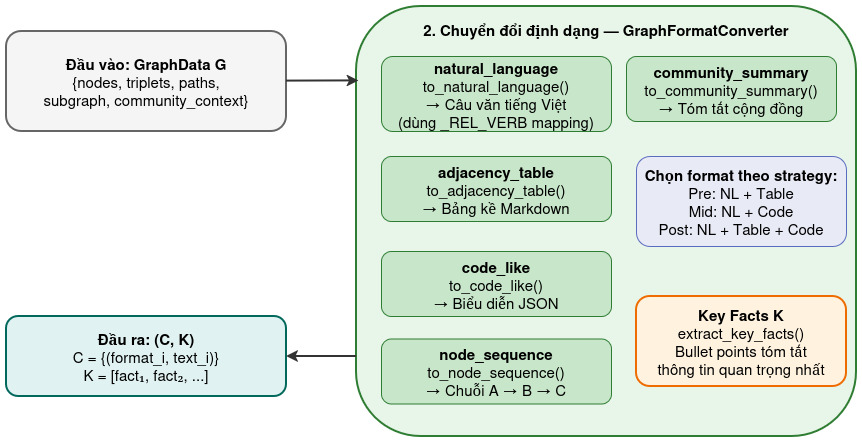
\includegraphics[width=\textwidth]{figures/c3/context_organization.jpg}
  \caption{Quy trình tổ chức ngữ cảnh.}
  \label{fig:context_organization}
\end{figure}
% ===========================================================
\subsection{Thiết kế phân hệ G-Generation}
\label{sec:g_generation}

Phân hệ G-Generation chịu trách nhiệm chuyển hoá ngữ cảnh tri thức đã được cung cấp từ phân hệ G-Retrieval thành câu trả lời ngôn ngữ tự nhiên thông qua mô hình ngôn ngữ lớn. Hệ thống được thiết kế để các câu trả lời của LLM có liên kết chặt chẽ với ngữ cảnh được cung cấp thay vì quá phụ thuộc vào tri thức nội tại của chúng, nhờ đó mà trong quá trình triển khai có thể thay thế chúng nhanh chóng mà không ảnh hưởng đến hiệu quả của pipeline.

Đầu vào tổng thể của phân hệ là bộ $(C, K, q)$ kế thừa trực tiếp từ đầu ra của giai đoạn Tổ chức ngữ cảnh; đầu ra là câu trả lời $a$ dưới dạng ngôn ngữ tự nhiên (Hình~\ref{fig:g_generation_overview}). Phân hệ được tổ chức thành hai giai đoạn xử lý tuần tự: bộ xây dựng prompt tổ hợp $(C, K, q)$ thành prompt hoàn chỉnh $\mathcal{P}$; sau đó bộ thực thi chiến lược tạo sinh gọi LLM dựa trên $\mathcal{P}$ để sinh ra $a$.

\begin{figure}[!ht]
  \centering
  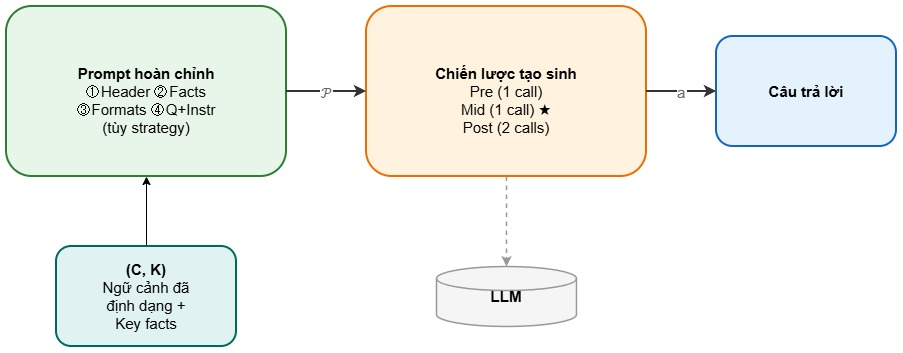
\includegraphics[width=\textwidth]{figures/c3/g_generation_overview.jpg}
  \caption{Sơ đồ tổng quan phân hệ G-Generation.}
  \label{fig:g_generation_overview}
\end{figure}


\subsubsection{Xây dựng cấu trúc Prompt}

LLM được sử dụng trong hệ thống không trải qua quá trình huấn luyện bổ sung (\textit{fine-tuning}) cho miền dữ liệu nghệ thuật Chèo, do đó toàn bộ tri thức miền cần được cung cấp ngay tại thời điểm tạo sinh câu trả lời thông qua prompt. Giai đoạn này đảm nhận việc tổ hợp ngữ cảnh đa định dạng $C$, dữ kiện chính $K$ và câu hỏi gốc $q$ thành một prompt hoàn chỉnh $\mathcal{P}$ theo cấu trúc cố định, sao cho LLM có thể tận dụng tối đa tri thức được cung cấp.

\textbf{Đầu vào.} Bộ $(C, K, q)$ từ giai đoạn Tổ chức ngữ cảnh.

\textbf{Cấu trúc prompt.} Prompt $\mathcal{P}$ gồm bốn thành phần tuần tự (Bảng~\ref{tab:prompt_structure}). Nguyên tắc thiết kế then chốt là đặt toàn bộ tri thức hỗ trợ trước câu hỏi- cách sắp xếp này phù hợp với cơ chế phân bổ trọng số chú ý của kiến trúc Transformer, vì mô hình có xu hướng tra cứu mạnh hơn tới các token xuất hiện trước trong chuỗi đầu vào khi suy luận. Riêng tập con định dạng từ $C$ được đưa vào ô ③ ``Khối ngữ cảnh'' không cố định, mà tuỳ theo chiến lược tạo sinh sẽ kích hoạt - chi tiết cơ chế chọn định dạng được trình bày ở Mục~\ref{sec:strategies}.

\begin{table}[ht]
  \centering
  \caption{Các thành phần cấu trúc prompt.}
  \label{tab:prompt_structure}
  \resizebox{\textwidth}{!}{%
  \begin{tabular}{c l l l}
    \hline
    \textbf{TT} & \textbf{Thành phần} & \textbf{Nội dung} & \textbf{Nguồn} \\
    \hline
    \textcircled{1} & Tiêu đề ngữ cảnh & ``Thông tin từ đồ thị tri thức về Chèo'' & Hằng số cố định \\
    \textcircled{2} & Dữ kiện chính & Tóm tắt dữ kiện quan trọng (dạng gạch đầu dòng) & $K$ từ G-Retrieval \\
    \textcircled{3} & Khối ngữ cảnh & Ngữ cảnh theo các định dạng được chọn & $C$ từ G-Retrieval \\
    \textcircled{4} & Câu hỏi + Chỉ dẫn & Câu hỏi và ràng buộc tạo sinh & Khuôn mẫu theo chiến lược \\
    \hline
  \end{tabular}%
  }
\end{table}

\textbf{Đầu ra.} Prompt $\mathcal{P}$ hoàn chỉnh, sẵn sàng gửi tới LLM. Với chiến lược Pre-Generation, prompt $\mathcal{P}$ cụ thể có dạng:

\begin{tcolorbox}[colback=gray!5, colframe=black!50, arc=4pt, boxrule=0.5pt, left=4pt, right=4pt, top=4pt, bottom=4pt]
{\small
\begin{verbatim}
# Thông tin từ đồ thị tri thức về Chèo      ← ①

## Tóm tắt quan trọng:                      ← ②
- Nhân vật: Thị Màu
- Diễn viên: Vân Quyền
- Vở: Quan Âm Thị Kính

## Mô tả tự nhiên:                          ← ③
Nhân vật Thị Màu thuộc vở diễn Quan Âm
Thị Kính và được thể hiện bởi Vân Quyền.

## Bảng quan hệ:                            ← ③
| Nút Bắt Đầu      | Quan Hệ        | Nút Đích          |
|------------------|----------------|-------------------|
| Quan Âm Thị Kính | HAS_CHARACTER  | Thị Màu           |
| Thị Màu          | PERFORMED_BY   | Vân Quyền         |

# Câu hỏi                                  ← ④
Ai đóng vai Thị Màu trong vở Quan Âm Thị Kính?

# Yêu cầu
Trả lời dựa trên thông tin đồ thị ở trên.
Nhớ trích dẫn cụ thể tên từ đồ thị.
\end{verbatim}
}
\end{tcolorbox}

\begin{figure}[ht]
  \centering
  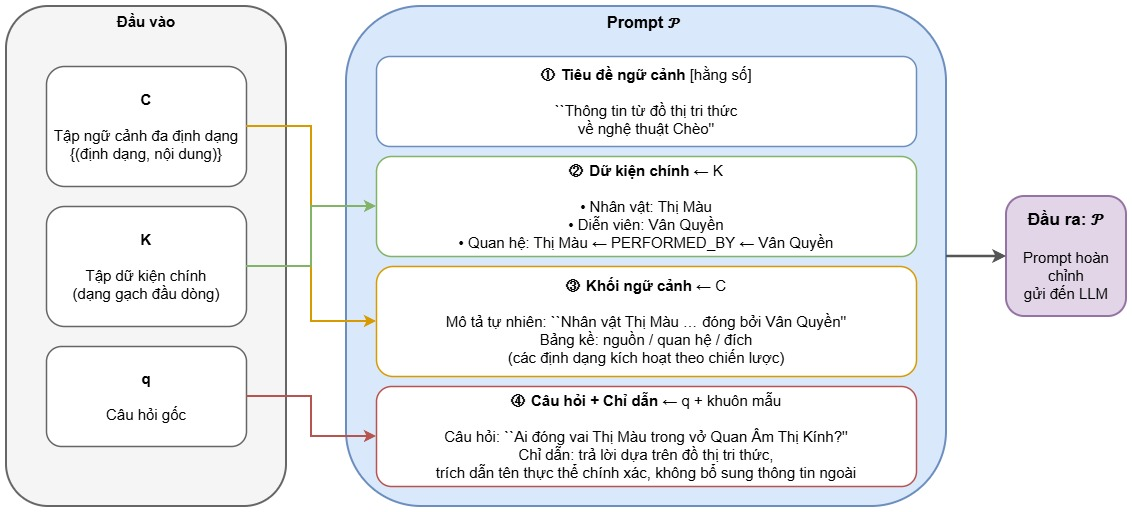
\includegraphics[width=0.85\textwidth]{figures/c3/prompt_structure.jpg}
  \caption{Cấu trúc các thành phần của prompt.}
  \label{fig:prompt_structure}
\end{figure}


\subsubsection{Các chiến lược tạo sinh}
\label{sec:strategies}

Phân hệ G-Generation triển khai ba chiến lược tạo sinh khác nhau ở mức độ kiểm soát quá trình suy luận của mô hình, số lượt gọi LLM và độ trễ. Ba chiến lược tạo thành một phổ liên tục - từ việc tận dụng năng lực nội tại của LLM với chi phí thấp, đến việc thêm ràng buộc cấu trúc cho suy luận, cũng như cơ chế kiểm định hậu kỳ - mỗi mức độ phù hợp với một dạng câu hỏi khác nhau.

\textbf{Đầu vào.} Prompt $\mathcal{P}$ từ giai đoạn xây dựng prompt cùng nhãn loại truy vấn $t$ từ giai đoạn tiền xử lý.

\textbf{Các chiến lược tạo sinh.} Ba chiến lược được mô tả lần lượt dưới đây.

\textit{Chiến lược Pre-Generation.} Toàn bộ ngữ cảnh truy xuất từ đồ thị tri thức được tổ chức và cung cấp trực tiếp cho mô hình trong một prompt duy nhất, sau đó LLM sinh câu trả lời ngay trong một lượt gọi. Mô hình ngôn ngữ được toàn quyền quyết định cách thức suy luận và định hướng câu trả lời của nó, không chịu ràng buộc về bất cứ cấu trúc suy luận hay logic nào cả. Do đó, hiệu quả của chiến lược phụ thuộc hoàn toàn vào chất lượng và độ rõ ràng của ngữ cảnh được chuẩn bị. Pre-Generation phù hợp với các truy vấn tra cứu trực tiếp, nơi quan hệ giữa thực thể đã rõ ràng trong dữ liệu, nhờ chi phí thấp và độ trễ nhỏ.

\textit{Chiến lược Mid-Generation.} Hệ thống áp một khuôn mẫu có cấu trúc lên prompt, buộc LLM thực hiện tuần tự ba bước: trích xuất dữ kiện, phân tích, và kết luận - mỗi kết luận phải được liên kết tường minh với bằng chứng từ ngữ cảnh. So với Pre-Generation, Mid-Generation đánh đổi một phần chi phí để tăng độ tin cậy, đặc biệt với các câu hỏi yêu cầu suy luận nhiều bước hoặc tổng hợp thông tin từ nhiều quan hệ trong đồ thị. Chiến lược này có nhiệm vụ khiến cho hành vi của LLM có kiểm soát hơn, tận dụng được tối đa các tri thức ngữ cảnh được cung cấp, từ đó sinh ra câu trả lời có giá trị hơn cả về ngữ nghĩa lẫn hình thức.

\textit{Chiến lược Post-Generation.} Chiến lược này bổ sung một bước kiểm định hậu kỳ nhằm phát hiện sai lệch trong câu trả lời. Ở lượt gọi thứ nhất, LLM sinh câu trả lời sơ bộ $a_0$ chỉ dựa trên tri thức tham số hoá (parametric knowledge) - không được cung cấp ngữ cảnh từ đồ thị tri thức. Ở lượt gọi thứ hai, $a_0$ được đối chiếu với ngữ cảnh từ đồ thị tri thức để phát hiện và hiệu chỉnh sai sót. Tách biệt giữa sinh và kiểm chứng cho phép phát hiện sự không nhất quán giữa tri thức nội tại của mô hình và dữ liệu thực tế, đổi lại chi phí tính toán và độ trễ lớn hơn hai chiến lược còn lại.

\begin{figure}[!ht]
  \centering
  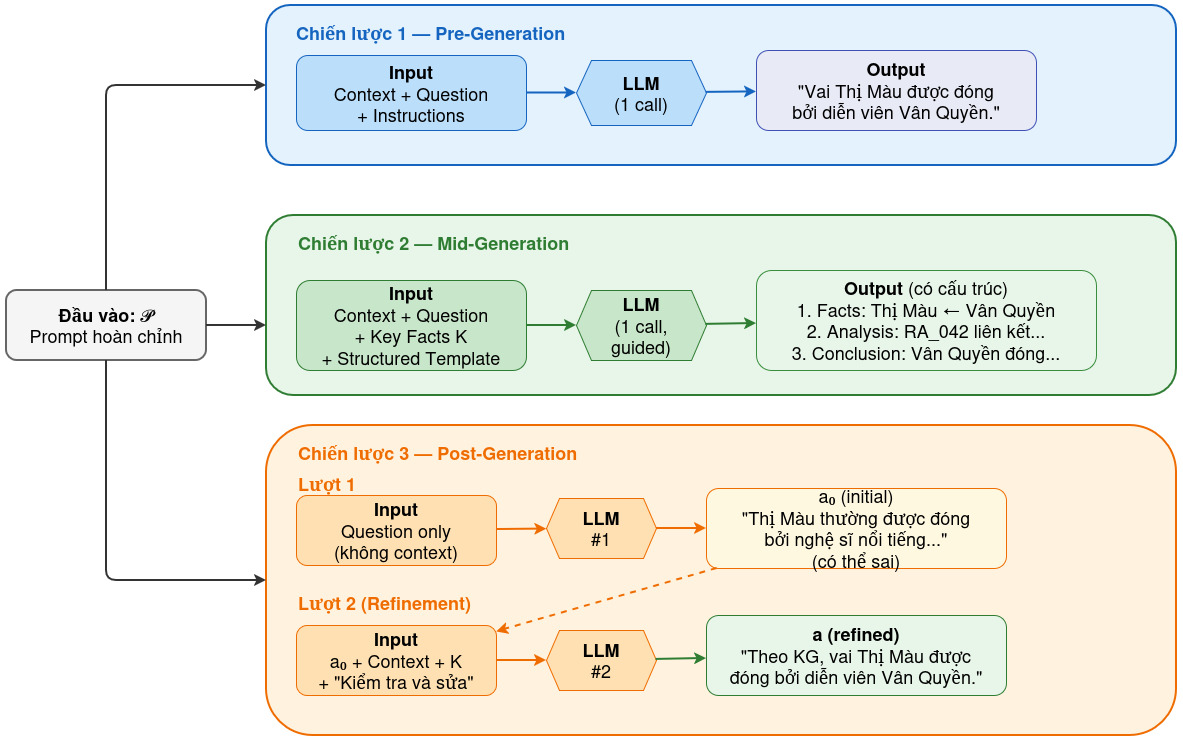
\includegraphics[width=\textwidth]{figures/c3/generation_strategies.jpg}
  \caption{Ba chiến lược tạo sinh.}
  \label{fig:generation_strategies}
\end{figure}

\textbf{Định tuyến chiến lược theo loại truy vấn.} Ba chiến lược được ánh xạ trực tiếp với nhãn $t$ đã sinh ở Tiến trình A của giai đoạn tiền xử lý (Bảng~\ref{tab:strategy_mapping}). Cùng cơ chế định tuyến với việc chọn mức truy xuất, ánh xạ này không phát sinh thêm độ trễ vì $t$ đã được tính sẵn. Mỗi chiến lược cũng kích hoạt một tập con định dạng từ $C$ phù hợp với cơ chế suy luận của mình: Pre-Generation dùng \texttt{natural\_language} và \texttt{adjacency\\\_table} cho việc tra cứu nhanh; Mid-Generation dùng \texttt{natural\_language} và \texttt{code\_like} để có thể bóc tách thuộc tính chi tiết khi phân tích; Post-Generation dùng đủ ba định dạng \texttt{natural\_language}, \texttt{adjacency\_table} và \texttt{code\_like} để có thêm cơ sở đối chiếu khi kiểm định ở lượt thứ hai.

\begin{table}[ht]
  \centering
  \caption{Ánh xạ chiến lược tạo sinh theo loại truy vấn.}
  \label{tab:strategy_mapping}
  \resizebox{\textwidth}{!}{%
  \begin{tabular}{l l p{8cm}}
    \hline
    \textbf{Loại truy vấn} & \textbf{Chiến lược} & \textbf{Lý do lựa chọn} \\
    \hline
    Local      & Pre-Generation  & Tra cứu trực tiếp; quan hệ đã rõ trong ngữ cảnh, ưu tiên độ trễ thấp. \\
    Community  & Mid-Generation  & Cần suy luận nhiều bước hoặc tổng hợp cụm quan hệ; khuôn mẫu cấu trúc giúp mô hình bám bằng chứng. \\
    Global     & Post-Generation & Tổng hợp xuyên vở, sai sót khó phát hiện; kiểm định hậu kỳ hạn chế ảo giác. \\
    \hline
  \end{tabular}%
  }
\end{table}

\textbf{Đầu ra.} Câu trả lời $a$ dưới dạng ngôn ngữ tự nhiên. Với $t = \textit{Local}$ kích hoạt chiến lược Pre-Generation, đầu ra cụ thể có dạng:

\begin{tcolorbox}[colback=gray!5, colframe=black!50, arc=4pt, boxrule=0.5pt]
{\small
\begin{verbatim}
a = "Theo dữ liệu đồ thị tri thức, vai nhân vật
     Thị Màu trong vở Quan Âm Thị Kính được đóng
     bởi diễn viên Vân Quyền."
\end{verbatim}
}
\end{tcolorbox}

Đầu ra của chiến lược Mid-Generation có cấu trúc ba bước tường minh:

\begin{tcolorbox}[colback=gray!5, colframe=black!50, arc=4pt, boxrule=0.5pt]
{\small
\begin{verbatim}
1. Thông tin từ đồ thị:
   - Nhân vật: Thị Màu
   - Diễn viên: Vân Quyền
   - Vở: Quan Âm Thị Kính
   - Quan hệ: Vân Quyền --PERFORMS--> Thị Màu

2. Phân tích:
   Theo dữ liệu đồ thị tri thức, nhân vật Thị Màu
   trong vở Quan Âm Thị Kính được thể hiện bởi
   diễn viên Vân Quyền.

3. Kết luận:
   Vai Thị Màu trong vở Quan Âm Thị Kính được
   đóng bởi diễn viên Vân Quyền.
\end{verbatim}
}
\end{tcolorbox}

Luồng xử lý của chiến lược Post-Generation chia thành hai lượt gọi:

\begin{tcolorbox}[colback=gray!5, colframe=black!50, arc=4pt, boxrule=0.5pt]
{\small
\begin{verbatim}
Lượt 1: Sinh câu trả lời sơ bộ a_0 chỉ dựa trên tri
        thức nội tại của LLM (không có ngữ cảnh từ
        đồ thị tri thức)

a_0 = "Vai Thị Màu trong vở Quan Âm Thị Kính đã được
       nhiều nghệ sĩ Chèo thể hiện qua các thế hệ.
       Tôi không chắc chắn về một diễn viên cụ thể
       trong dữ liệu của tôi."

  → a_0 mơ hồ vì LLM không có dữ liệu xác thực,
    không trích dẫn được tên diễn viên cụ thể


Lượt 2: Đối chiếu a_0 với ngữ cảnh C và dữ kiện K
        từ đồ thị tri thức để bổ sung và hiệu chỉnh

K = ["Nhân vật: Thị Màu",
     "Diễn viên: Vân Quyền",
     "Vở kịch: Quan Âm Thị Kính",
     "Quan hệ diễn xuất: Thị Màu ← Vân Quyền", ...]

a = "Theo dữ liệu đồ thị tri thức, vai nhân vật
     Thị Màu trong vở Quan Âm Thị Kính được đóng
     bởi diễn viên Vân Quyền."

  → a được hiệu chỉnh, bổ sung dữ kiện cụ thể từ
    đồ thị thay cho câu trả lời mơ hồ ở lượt 1
\end{verbatim}
}
\end{tcolorbox}